\section{岭回归}
\subsection{模型介绍}
岭回归是在基础的线性回归模型的损失函数上,增加了L2正则项,同样假设有p个预测变量,此时Lasso损失函数如下:
\begin{equation}
 \sum_{i=1}^n(y_i-\beta^Tx_i)^2+\lambda\sum_{j=1}^p\beta_j^2
\end{equation}
由于岭回归的损失函数可导,所以也可以直接求解出一个回归系数的估计值为$\hat{\beta}=(X^TX+\lambda I)^{-1}XY$,随着 $\lambda$的增大,$(X^TX+\lambda I)^{-1}$就越小,模型的方差就越小;而$\lambda$越大使得 $\beta$的估计值更加偏离真实值,模型的偏差就越大。所以岭回归的关键是找到一个合理的 $\lambda$值来平衡模型的方差和偏差。

\subsection{自己实现的岭回归与自带包实现的岭回归}
这里我们先比较自己实现的岭回归的参数估计与自带包实现的参数。首先选取超参数$\lambda$为$0.01$,使用两种不同的代码实现岭回归,得到模型中的参数如下表。我们可以看到两者系数相差无几,而之前lasso自己编写的代码和自带包估计的系数差距较大,我们分析认为是岭回归同样能得到模型的解析解,可以直接用数据来计算得到每个超参数下系数的最优估计,所以在岭回归方面,我们自己编写的岭回归参数估计与R中自带包计算的效果几乎相同。

\begin{table}[htbp]
\centering
\caption{自己编写与R包用岭回归方法估计系数的结果}
\begin{tabular}{ccccccccccccccc}
  \hline
 & 截距项 & crim & zn & indus & chas & nox & rm & age & dis & rad & tax & ptratio & black & lstat \\ 
  \hline
  手写代码 & 35.96 & -0.11 & 0.05 & 0.02 & 2.69 & -17.48 & 3.83 & 0.00 & -1.47 & 0.30 & -0.01 & -0.95 & 0.01 & -0.52 \\ 
  自带包& 36.46 & -0.11 &  0.05 &  0.02  & 2.69 &-17.76 &3.81  & 0.00&  -1.48&   0.31 & -0.01&  -0.95&0.01&-0.52\\
   \hline
\end{tabular}
\end{table}

\subsection{基于交叉验证选择最佳参数}

自动选择参数$\lambda$值的范围进行岭回归,选择在 $\lambda =10^{-3}$到 $\lambda = 10$的范围内进行岭回归,如图所示可得每个变量的系数随着参数$\lambda$变化所得到的曲线.该图上方的13是系数个数,而下方10,15,20,25是每个$\lambda$的值对应的各变量参数的绝对值之和。我们可以从图的左端看出,即使各个变量系数的值都接近到0,但在图像上方对应的值仍为13,说明岭回归没有变量选择的作用,只会随着$\lambda$值增加,而压缩各变量系数的值。
\begin{figure}[htbp]
  \centering
  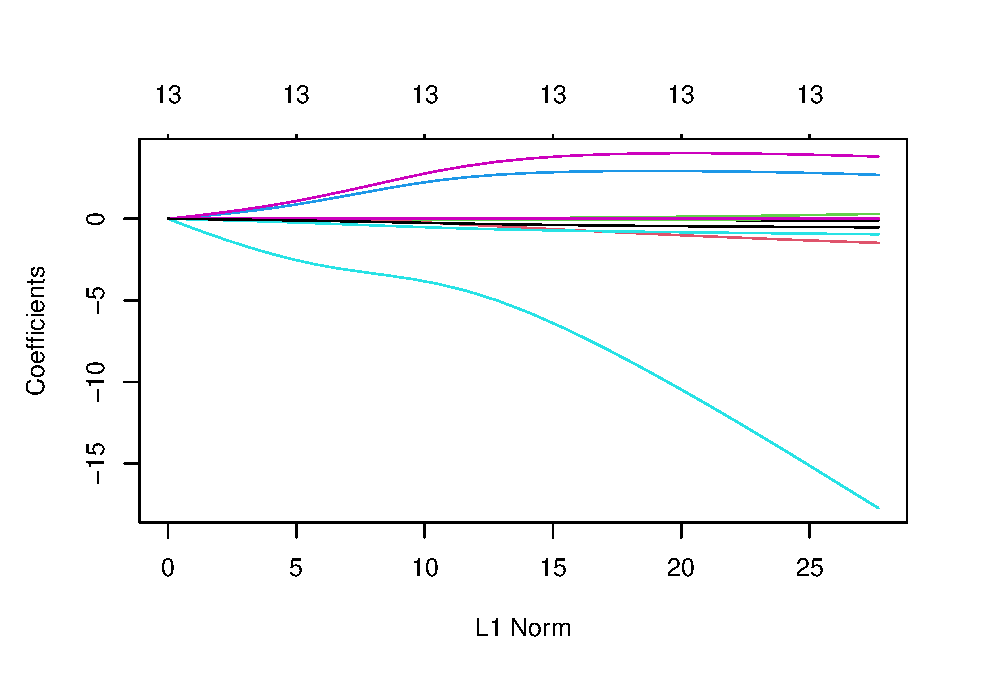
\includegraphics[width=0.8\textwidth]{opt_para.eps}
  \caption{系数变化曲线}
\end{figure}

将数据分为10折,使用交叉验证法选择调节参数$\lambda$,得到系数变化曲线如图3所示
\begin{figure}[htbp]
  \centering
  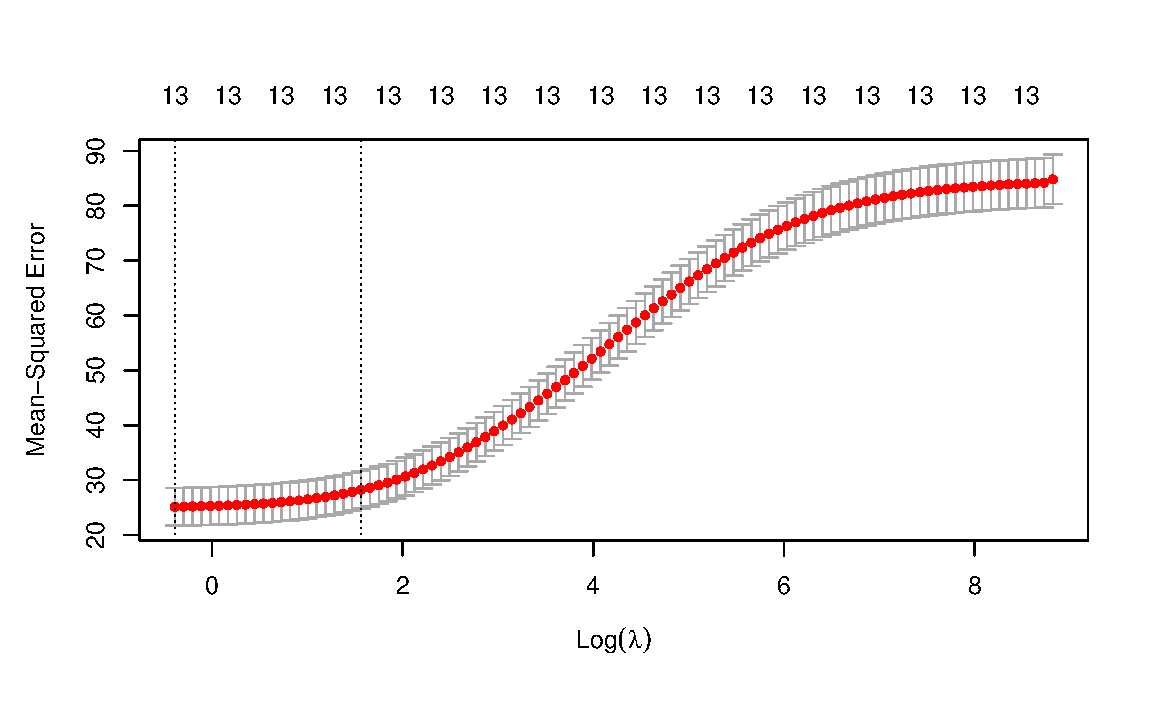
\includegraphics[width=0.6\textwidth]{cv_para.eps}
  \caption{交叉验证法的系数变化曲线}
\end{figure}

我们分别选取$\lambda$的LSE值以及最小的$\lambda$值下的变量系数,结果如图4所示,数据第一列是$\lambda$的LSE值对应的变量系数,第二列是CV准则下最小MSE的$\lambda$值下的变量系数。
\begin{figure}[htbp]
  \centering
  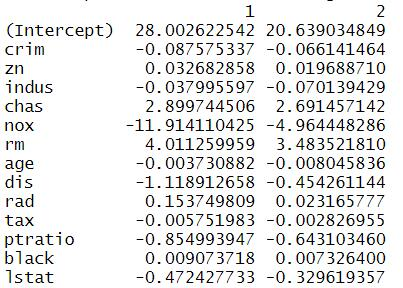
\includegraphics[width=0.6\textwidth]{coef.jpg}
  \caption{两个$\lambda$值下的系数}
\end{figure}
